% =============================================================================
% =============================================================================
% =============================================================================
\section{The Near-Earth Environment}

From Earth's surface up to about $\sim\SI{100}{\km}$, the atmosphere is a well-behaved fluid: a collisional ensemble of neutral atoms. However, beyond there, its behavior changes dramatically. As altitude increases, solar ultraviolet radiation becomes more intense, which ionizes atmospheric atoms. Density also decreases, slowing collisional recombination. Whereas the neutral atmosphere is held against Earth's surface by gravity, the behavior of charged particles is dominated by Earth's geomagnetic field... and the electromagnetic disturbances created as that field is hammered by the solar wind. 

The present section outlines the structure of several features between the magnetopause current sheet and the ionospheric current sheet which are relevant to the investigation at hand. 

... \\ \\

6.6RE is geosynchronous. 

60RE is the moon. 

Tail goes back to 100RE or so. 

\todo{Sketch out the goneral structure of the magnetosphere, from the ionospheric current sheet (is this too generous?) to the magnetopause (a real current sheet). Talk about where gravity dominates, where field line curvature becomes apparent, and where the moon sits in all this. }

From \cite{paschmann_2003}: ``In the thermosphere, the solar ultraviolet (UV) light and energetic particles precipitating from the magnetosphere produce ionization increasing with altitude. At the same time the particle density is low enough to make the recombination times of the ionized atoms and molecules sufficiently long to allow a significant fraction of the gas to remain ionized. This produces a conducting layer of the atmosphere known as the ionosphere. The ionosphere begins at $\sim\SI{65}{\km}$, has a peak plasma density between 200 and 300 km, and eventually merges with magnetospheric regions $\sim$1000--2000 km altitudes.''

The ionospheric E region is collisionally coupled to the neutrals. This decouples the ion and electron drifts, allowing currents to flow perpendicular to the magnetic field. 

\todo{\Alfven waves couple the magnetosphere to the ionosphere\cite{paschmann_2003}. Waves travel down the field line, accelerating particles to match the magnetospheric driver (for example, increased flow velocity as a result of enhanced reconnection). Bounces off of the ionosphere. May also bounce off the driver. Builds up drag and brings about equilibrium. }


At 10**5 km, the bow shock. On the dayside, at least. Balance between Earth's magnetic field and that of the sun. Another current sheet... This one far more intense.

Still less than halfway to the moon. That's 3e5 km.

This with is concerned with the behavior of electromagnetic waves that propagate inside the magnetosheath, but outside the ionosphere; in fact, they play a significant role in the transport of energy from the former to the latter. 

Free electron density... Still mostly neutrals, but collisions are so rare that they don't matter. At x, the mean free path of a neutral atom is comparable to... 

%There are a lot of interrelated things going on, so it's hard to describe Earth's environment one step at a time. Look at Scott's thesis -- he did this well, right? 

%Heliosphere, Magnetosphere, Ionosphere, Atmosphere?

%Typical solar wind density is $\sim$ \SI{5}{/\cm\cubed}. Typical solar wind velocity at Earth is \SIrange{e2}{e3}{\km/\s}. Typical solar wind particle energy is \SIrange{1}{10}{\kilo\eV}. Density can vary by $\sim$3 orders of magnitude, and velocity by one, during times of high solar activity. CMEs can also mess with the north/south component of the interplanetary magnetic field. 

At Earth's orbit, the solar magnetic field makes more-or-less a \SI{45}{\degree} angle with the \X axis. 
\footnote{Uppercase \X, \Y, and \Z are used to indicate GSE coordinates: \X points from the Earth to the Sun; \Y is perpendicular to \X in the Sun's ecliptic plane, pointing duskwards; \Z points north, out of the ecliptic plane. In later chapters, lowercase \x, \y, and \z are used to define a more-or-less analogous corodinate system with respect to Earth. }

% Solar wind is what deforms Earth's magnetic field to form the magnetosphere. 

% Transient solar wind phenomena, such as coronal mass ejections, are also known to be related to geomagnetic disturbances at Earth. Jesse cites here: 

% R. L. McPherron. Physical processes producing magnetospheric substorms and mangetic storms. In J. A. Jacobs, editor, Geomagnetism, volume 4, chapter 7. Academic Press, 1991.

% G. Rostoker. Substorms. In Handbook of the Solar-Terrestrial Environment, chapter 15. Springer-Verlag, 2007.

% This might just be worth tracking down... Jesse cites several chapters: 

% M. Shulz. Magnetospheres. In Handbook of the Solar-Terrestrial Environment, chapter 7. Springer-Verlag, 2007.

% papers mentioned during Yan's talk. mostly about alfven acceleration and nonlinear effects. 
% Vasyliunas 1970, 1984
% Hasegawa 1976
% Goertz 1991
% Stasiewicz et al 2000
% Haerendel 2008
% Song & Lysak 1994, 1999, 2000, 2001, 2006, 2011, 2012
% Inverted V?
% Double layers? 
% Charge holes? 

% -----------------------------------------------------------------------------
% -----------------------------------------------------------------------------
% -----------------------------------------------------------------------------
\subsection{The Outer Magnetosphere}

Significant deformation by the solar wind. 

Bow shock. 

Magnetopause. Current sheet consistent with \amplaw. 

Plasma sheet and PSBL. 

Tail and tail lobes. 

Reconnection. 

% -----------------------------------------------------------------------------
% -----------------------------------------------------------------------------
% -----------------------------------------------------------------------------
\subsection{The Inner Magnetosphere}

Closed field lines. More or less dipolar. 

The plasmasphere and plasmapause. 

Radiation belts. Radial diffusion is interesting because... 

\Alfven speed. So we probably want to at least mention field line resonance here? Or do we get into that in the next chapter? Plot of \Alfven speeds and \Alfven bounce times for each profile. 

% -----------------------------------------------------------------------------
% -----------------------------------------------------------------------------
% -----------------------------------------------------------------------------
\subsection{The Ionosphere}
  \label{sec_ionos}



One hundred kilometers above Earth's surface, give or take, the neutral atmosphere transitions into the conducting ionosphere. Solar ultraviolet radiation is intense enough -- and collisional recombination slow enough -- to maintain a sizable density of charged particles. Moreover, collisions are common enough to disrupt the plasma's frozen-in condition\footnote{In a collisionless plasma, charged particles move freely along magnetic field lines, but cannot cross magnetic field lines; as a result, a compression in the plasma is synonymous to a compression of the plasma that threads it. }, allowing current to flow perpendicular to Earth's dipole magnetic field. 


In the ionosphere ($\sim\SIrange{e2}{e4}{\km}$), solar ultraviolet radiation is intense enough -- and collisional recombination slow enough -- to maintain a sizable density of charged particles. 







This marks the transition between the neutral atmosphere (a well-mixed fluid dominated by Earth's gravity) to the magnetosphere (a structured plasma with behavior governed by electromagnetic fields). 

The nitrogen density (w at sea level) drops from x at 100km to y at 1000km to z at 10**4 km.


Pedersen, Hall, and field-aligned conductivity. Do we want to get into two-cell convection? Region 1 and 2 current? 

\todo{Convection electric field. How close to Earth does it get? Don't we lose $\vec{E}=\cross{V}{B}$ when there are currents? }

``Increasing the Hall conductance allows the energy to oscillate through the inductive process rather than dissipate as Joule heating, increasing the `ringtime' of field line resonances.''\cite{waters_2013}

Scale heights. Ion/neutral composition. 

E, F layers. 

Ionospheric \Alfven resonator. This is important if we want to talk briefly about all kinds of ULF waves. 

Precipitation. Inverted V. 

\todo{Scott's thesis has a TON of detail. How much does Jesse show? }

\begin{figure}[H]
    \centering
    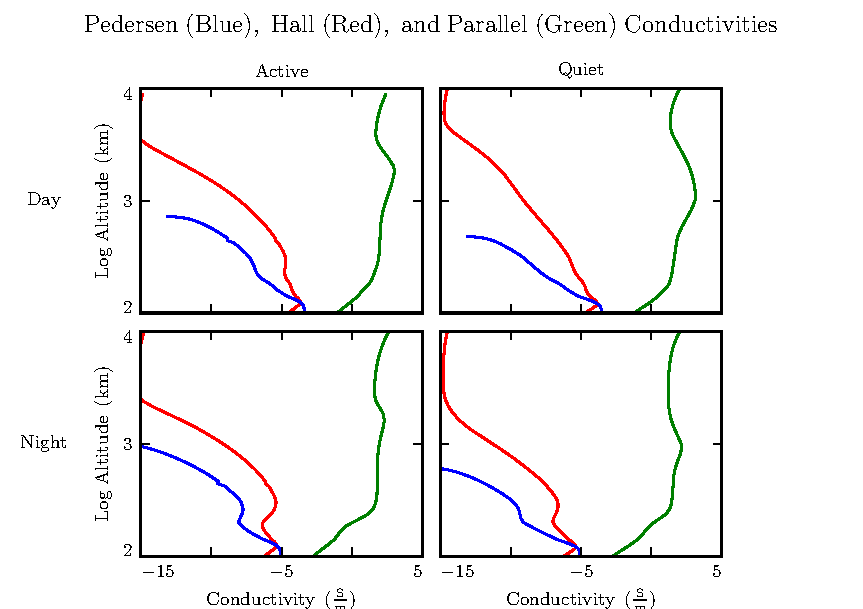
\includegraphics[width=\textwidth]{figures/sigma.pdf}
    \caption[Ionospheric Conductivity Profiles]{
      Ionospheric conductivity profiles, adapted by Lysak\cite{lysak_2013} from Appendix B of Kelley's textbook\cite{kelley_1989}. 
    }
    \label{fig_sigma}
\end{figure}


\begin{longtable}{ @{\extracolsep{\fill}} lrrr @{\extracolsep{\fill}} }
  \caption[Integrated Atmospheric Conductivity]{Integrated Atmospheric Conductivity (\si{\S})}
  \label{tab_sigma_atm} \\

  \toprule
  &
  $\Sigma_0$ &
  $\Sigma_P$ &
  $\Sigma_H$ \\
  \midrule
  \endfirsthead

  % Footer for the end of the table
  \bottomrule
  \endlastfoot

  Active Day &
  424 &
  0.65 &
  6.03 \\

  Quiet Day &
  284 &
  0.44 &
  4.02 \\

  Active Night &
  9 &
  0.01 &
  0.12 \\

  Quiet Night &
  9 &
  0.01 &
  0.12 \\

\end{longtable}

\begin{longtable}{ @{\extracolsep{\fill}} lrrr @{\extracolsep{\fill}} }
  \caption[Integrated Ionospheric Conductivity]{Integrated Ionospheric Conductivity (\si{\S})}
  \label{tab_sigma_ionos} \\

  \toprule
  &
  $\Sigma_0$ &
  $\Sigma_P$ &
  $\Sigma_H$ \\
  \midrule
  \endfirsthead

  % Footer for the end of the table
  \bottomrule
  \endlastfoot

  Active Day &
  --- &
  13.0 &
  17.0 \\

  Quiet Day &
  --- &
  5.6 &
  10.2 \\

  Active Night &
  --- &
  0.8 &
  0.3 \\

  Quiet Night &
  --- &
  0.2 &
  0.3 \\

\end{longtable}


\todo{Get this working... }


